% Figure: service architecture -- sources, the vi-dbpedia-data pipeline,
% the published Linked Data and the Fuseki query service (docker-compose.yml).
\documentclass[tikz, border=4mm]{standalone}
% Shared style for the project figures. Compile each figure with XeLaTeX.
% Notation follows the IE650 Knowledge Graphs slides (University of Mannheim):
%   resource (IRI) = ellipse, literal = rectangle, labelled arrow = property,
%   unlabelled arrow = rdfs:subClassOf ("convention for this course").
\usepackage{fontspec}
% TeX Gyre Heros/Cursor: Helvetica/Courier clones with Vietnamese letters.
\setmainfont{texgyreheros}[
  Extension=.otf, UprightFont=*-regular, BoldFont=*-bold,
  ItalicFont=*-italic, BoldItalicFont=*-bolditalic]
\setmonofont{texgyrecursor}[
  Extension=.otf, UprightFont=*-regular, BoldFont=*-bold,
  ItalicFont=*-italic, BoldItalicFont=*-bolditalic]
\renewcommand{\familydefault}{\sfdefault}
\usetikzlibrary{arrows.meta, calc, fit, positioning, backgrounds,
  shapes.geometric, shapes.misc}

\definecolor{kgfill}{HTML}{FCD5B0}     % node fill used in the lecture slides
\definecolor{kgline}{HTML}{8C8C8C}
\definecolor{kgnavy}{HTML}{0B2D50}     % arrows and dbo:/W3C property labels
\definecolor{kgnew}{HTML}{C0392B}      % new terms of this project (vio:)
\definecolor{kgextfill}{HTML}{D9E8F6}  % resources of other datasets (5th star)
\definecolor{kgext}{HTML}{2E75B6}
\definecolor{kgbox}{HTML}{F4F6F8}
\definecolor{kgmuted}{HTML}{5F6B76}

\tikzset{
  every picture/.style={line join=round},
  res/.style={ellipse, draw=kgline, fill=kgfill, font=\ttfamily,
    inner xsep=1pt, inner ysep=2pt, minimum height=9.5mm},
  cls/.style={res},
  lit/.style={rectangle, draw=kgline, fill=kgfill, font=\ttfamily,
    inner xsep=5pt, minimum height=8.5mm},
  ext/.style={res, draw=kgext, fill=kgextfill},
  rel/.style={-{Stealth[length=3mm, width=2.4mm]}, draw=kgnavy, line width=1pt},
  sub/.style={rel},
  nodomain/.style={rel, dash pattern=on 4.5pt off 2.5pt},
  lbl/.style={font=\ttfamily, text=kgnavy, fill=white, inner sep=1.2pt},
  newlbl/.style={lbl, text=kgnew},
  note/.style={font=\small, text=kgmuted, align=left},
  panel/.style={draw=kgline, fill=kgbox, rounded corners=2pt, inner sep=6pt},
  heading/.style={font=\bfseries, text=kgnavy, anchor=north west},
}

\usetikzlibrary{shapes.symbols}
\tikzset{
  cmdbox/.style={rectangle, rounded corners=2pt, draw=kgnavy, fill=white, line width=0.8pt,
    text width=6.3cm, align=left, inner sep=4pt},
  human/.style={cmdbox, dash pattern=on 4pt off 2pt, draw=kgmuted, text width=3.9cm},
  src/.style={rectangle, rounded corners=2pt, draw=kgline, fill=kgbox, text width=3.9cm,
    align=center, inner sep=5pt},
  lod/.style={ellipse, draw=kgext, fill=kgextfill, align=center, inner sep=0pt,
    minimum height=13mm},
  file/.style={tape, tape bend top=none, draw=kgline, fill=kgfill, align=center,
    text width=4.4cm, inner sep=3pt, font=\small},
  store/.style={cylinder, shape border rotate=90, aspect=0.22, draw=kgnavy, fill=kgfill,
    line width=0.8pt, align=center, minimum width=4.6cm, minimum height=2.5cm},
  client/.style={src, fill=white, text width=2.6cm},
  flow/.style={-{Stealth[length=2.6mm, width=2.1mm]}, draw=kgnavy, line width=0.9pt},
  proto/.style={font=\footnotesize, text=kgnavy, inner sep=1.5pt, align=center},
  lane/.style={draw=kgline!60, fill=kgbox!55, rounded corners=4pt},
  lanetitle/.style={font=\bfseries\small, text=kgnavy, anchor=north west, inner sep=3pt},
}
\newcommand{\cmd}[2]{\texttt{\textbf{#1}}\\[-1pt]{\small #2}}
\newcommand{\out}[1]{{\footnotesize\color{kgmuted}\texttt{→ #1}}}
\begin{document}
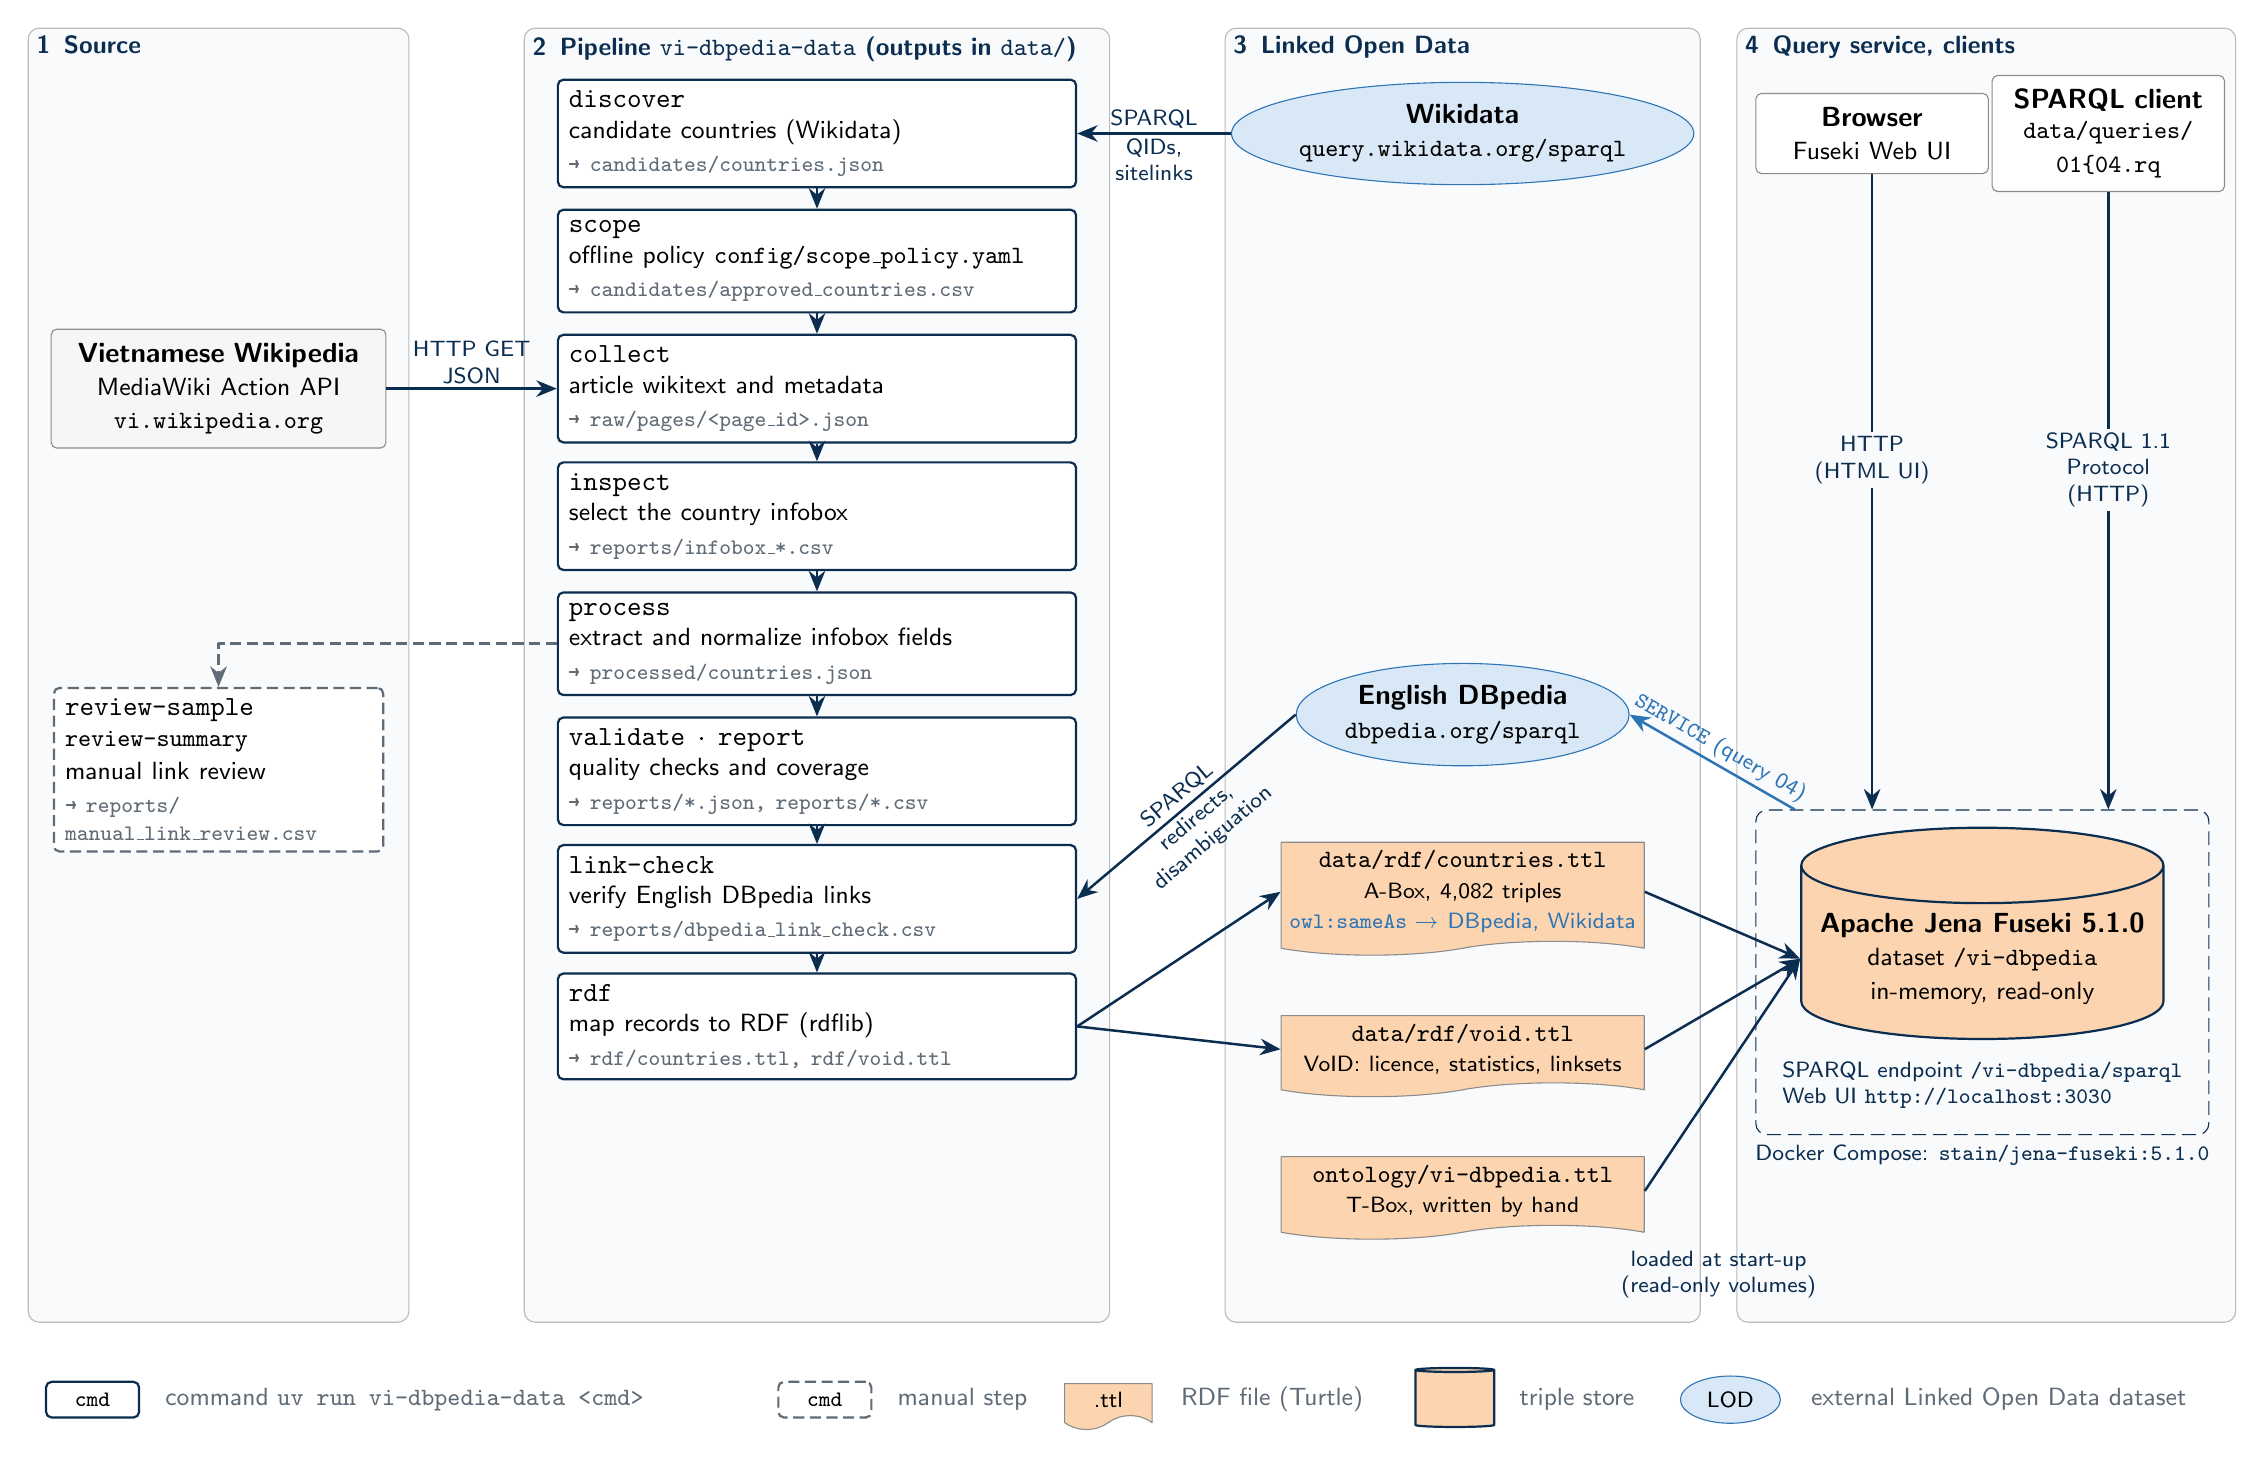
\begin{tikzpicture}

% ---- 2: extraction and transformation pipeline (CLI commands, in run order)
\foreach \i/\name/\text in {
  1/discover/{\cmd{discover}{candidate countries (Wikidata)}\\\out{candidates/countries.json}},
  2/scope/{\cmd{scope}{offline policy \texttt{config/scope\_policy.yaml}}\\\out{candidates/approved\_countries.csv}},
  3/collect/{\cmd{collect}{article wikitext and metadata}\\\out{raw/pages/<page\_id>.json}},
  4/inspect/{\cmd{inspect}{select the country infobox}\\\out{reports/infobox\_*.csv}},
  5/process/{\cmd{process}{extract and normalize infobox fields}\\\out{processed/countries.json}},
  6/validate/{\cmd{validate · report}{quality checks and coverage}\\\out{reports/*.json, reports/*.csv}},
  7/linkcheck/{\cmd{link-check}{verify English DBpedia links}\\\out{reports/dbpedia\_link\_check.csv}},
  8/rdf/{\cmd{rdf}{map records to RDF (rdflib)}\\\out{rdf/countries.ttl, rdf/void.ttl}}} {
  \node[cmdbox] (\name) at (9.8, 13.0 - 1.62*\i) {\text};
}
\foreach \a/\b in {discover/scope, scope/collect, collect/inspect, inspect/process,
    process/validate, validate/linkcheck, linkcheck/rdf} {
  \draw[flow] (\a) -- (\b);
}

% ---- 1: data source and the manual step
\node[src] (wiki) at (2.2, 8.14)
  {\textbf{Vietnamese Wikipedia}\\{\small MediaWiki Action API}\\\texttt{\small vi.wikipedia.org}};
\draw[flow] (wiki.east) -- node[proto, above] {HTTP GET\\JSON} (wiki.east -| collect.west);
\node[human] (review) at (2.2, 3.3)
  {\cmd{review-sample}{\textbf{\texttt{review-summary}}}\\{\small manual link review}\\
   \out{reports/}\\[-2pt]{\footnotesize\color{kgmuted}\texttt{manual\_link\_review.csv}}};
\draw[flow, dash pattern=on 4pt off 2pt, draw=kgmuted] (process.west) -| (review.north);

% ---- 3: Linked Open Data sources and the published dataset
\node[lod] (wikidata) at (18.0, 11.38)
  {\textbf{Wikidata}\\\texttt{\small query.wikidata.org/sparql}};
\draw[flow] (wikidata.west) -- node[proto, above] {SPARQL}
  node[proto, below] {QIDs,\\sitelinks} (wikidata.west -| discover.east);
\node[lod] (dbpedia) at (18.0, 4.0)
  {\textbf{English DBpedia}\\\texttt{\small dbpedia.org/sparql}};
\draw[flow] (dbpedia.west) -- node[proto, above, sloped] {SPARQL}
  node[proto, below, sloped] {redirects,\\disambiguation} (linkcheck.east);

\node[file] (data) at (18.0, 1.75)
  {\texttt{data/rdf/countries.ttl}\\{\footnotesize A-Box, 4,082 triples}\\
   {\footnotesize\color{kgext}\texttt{owl:sameAs} → DBpedia, Wikidata}};
\node[file] (void) at (18.0, -0.25)
  {\texttt{data/rdf/void.ttl}\\{\footnotesize VoID: licence, statistics, linksets}};
\node[file] (onto) at (18.0, -2.05)
  {\texttt{ontology/vi-dbpedia.ttl}\\{\footnotesize T-Box, written by hand}};
\draw[flow] (rdf.east) -- (data.west);
\draw[flow] (rdf.east) -- (void.west);

% ---- 4: query service (docker-compose.yml) and clients
\node[store] (fuseki) at (24.6, 0.9)
  {\textbf{Apache Jena Fuseki 5.1.0}\\{\small dataset \texttt{/vi-dbpedia}}\\{\small in-memory, read-only}};
\node[font=\footnotesize, text=kgnavy, align=left, anchor=north] (endpoints)
  at ($(fuseki.south) + (0, -0.15)$)
  {SPARQL endpoint \texttt{/vi-dbpedia/sparql}\\Web UI \texttt{http://localhost:3030}};
\node[draw=kgnavy, dash pattern=on 5pt off 2.5pt, rounded corners=4pt, inner sep=6pt,
  fit=(fuseki) (endpoints)] (container) {};
\node[font=\footnotesize, text=kgnavy, align=center, anchor=north] at (container.south)
  {Docker Compose: \texttt{stain/jena-fuseki:5.1.0}};
\foreach \f in {data, void, onto} {
  \draw[flow] (\f.east) -- (fuseki.west);
}
\node[proto, anchor=north] at (21.25, -2.75) {loaded at start-up\\(read-only volumes)};
\draw[flow, draw=kgext] ($(container.north west) + (0.5, 0)$) -- node[proto, sloped, above, text=kgext]
  {\texttt{SERVICE} (query 04)} (dbpedia.east);

\node[client] (browser) at (23.2, 11.38) {\textbf{Browser}\\{\small Fuseki Web UI}};
\node[client] (cli) at (26.2, 11.38)
  {\textbf{SPARQL client}\\{\small \texttt{data/queries/}\\\texttt{01–04.rq}}};
\draw[flow] (browser.south) -- node[proto, fill=kgbox!55, pos=0.45] {HTTP\\(HTML UI)}
  (browser.south |- container.north);
\draw[flow] (cli.south) -- node[proto, fill=kgbox!55, pos=0.45] {SPARQL 1.1\\Protocol\\(HTTP)}
  (cli.south |- container.north);

% ---- Lanes (background)
\begin{scope}[on background layer]
  \node[lane, fit={(-0.1, 12.6) (4.5, -3.6)}] (lane1) {};
  \node[lane, fit={(6.2, 12.6) (13.4, -3.6)}] (lane2) {};
  \node[lane, fit={(15.1, 12.6) (20.9, -3.6)}] (lane3) {};
  \node[lane, fit={(21.6, 12.6) (27.7, -3.6)}] (lane4) {};
\end{scope}
\node[lanetitle] at (lane1.north west) {1\enspace Source};
\node[lanetitle] at (lane2.north west) {2\enspace Pipeline \texttt{vi-dbpedia-data} (outputs in \texttt{data/})};
\node[lanetitle] at (lane3.north west) {3\enspace Linked Open Data};
\node[lanetitle] at (lane4.north west) {4\enspace Query service, clients};

% ---- Legend
\begin{scope}[shift={(0, -4.7)}]
  \node[cmdbox, text width=0.9cm, align=center, font=\footnotesize] at (0.6, 0) {\texttt{cmd}};
  \node[note, anchor=west] at (1.4, 0) {command \texttt{uv run vi-dbpedia-data <cmd>}};
  \node[human, text width=0.9cm, align=center, font=\footnotesize] at (9.9, 0) {\texttt{cmd}};
  \node[note, anchor=west] at (10.7, 0) {manual step};
  \node[file, text width=0.9cm, font=\footnotesize] at (13.5, 0) {.ttl};
  \node[note, anchor=west] at (14.3, 0) {RDF file (Turtle)};
  \node[store, minimum width=1.0cm, minimum height=0.75cm] at (17.9, 0) {};
  \node[note, anchor=west] at (18.6, 0) {triple store};
  \node[lod, minimum height=6mm, font=\footnotesize] at (21.4, 0) {\enspace LOD\enspace};
  \node[note, anchor=west] at (22.3, 0) {external Linked Open Data dataset};
\end{scope}

\end{tikzpicture}
\end{document}
